\documentclass[conference]{IEEEtran}
\IEEEoverridecommandlockouts
% The preceding line is only needed to identify funding in the first footnote. If that is unneeded, please comment it out.
\usepackage{cite}
\usepackage{amsmath,amssymb,amsfonts}
\usepackage{algorithmic}
\usepackage{graphicx}
\usepackage{textcomp}
\usepackage{xcolor}
\usepackage{cleveref}\usepackage{algorithm}
\usepackage{algpseudocode}
\usepackage{booktabs}
\usepackage{multirow}
\usepackage{tcolorbox}
\usepackage{enumitem}
\usepackage{adjustbox}
\usepackage{url}
\def\BibTeX{{\rm B\kern-.05em{\sc i\kern-.025em b}\kern-.08em
  T\kern-.1667em\lower.7ex\hbox{E}\kern-.125emX}}
\begin{document}

\title{Food Production Optimization
\thanks{Identify applicable funding agency here. If none, delete this.}
}

\author{\IEEEauthorblockN{1\textsuperscript{st} Given Name Surname}
\IEEEauthorblockA{\textit{dept. name of organization (of Aff.)} \\
\textit{name of organization (of Aff.)}\\
City, Country \\
email address or ORCID}
\and
\IEEEauthorblockN{2\textsuperscript{nd} Given Name Surname}
\IEEEauthorblockA{\textit{dept. name of organization (of Aff.)} \\
\textit{name of organization (of Aff.)}\\
City, Country \\
email address or ORCID}
\and
\IEEEauthorblockN{3\textsuperscript{rd} Given Name Surname}
\IEEEauthorblockA{\textit{dept. name of organization (of Aff.)} \\
\textit{name of organization (of Aff.)}\\
City, Country \\
email address or ORCID}
\and
\IEEEauthorblockN{4\textsuperscript{th} Given Name Surname}
\IEEEauthorblockA{\textit{dept. name of organization (of Aff.)} \\
\textit{name of organization (of Aff.)}\\
City, Country \\
email address or ORCID}
\and
\IEEEauthorblockN{5\textsuperscript{th} Given Name Surname}
\IEEEauthorblockA{\textit{dept. name of organization (of Aff.)} \\
\textit{name of organization (of Aff.)}\\
City, Country \\
email address or ORCID}
\and
\IEEEauthorblockN{6\textsuperscript{th} Given Name Surname}
\IEEEauthorblockA{\textit{dept. name of organization (of Aff.)} \\
\textit{name of organization (of Aff.)}\\
City, Country \\
email address or ORCID}
}

\maketitle


\begin{abstract}


Food production is the process by which land, water, labor, and other inputs are coordinated to generate the nutrients that sustain human populations -- and optimizing it at scale is one of the defining resource allocation challenges of the coming decades, as rising demand, climate volatility, and sustainability constraints simultaneously tighten.

We study a multi-objective crop allocation problem balancing nutritional value, environmental sustainability, and affordability for 27 distinct crops. We thereby evaluate the engineering and mathematical trade-offs of mapping large-scale structured tasks to quantum annealing hardware. The problem is modeled as a Binary Plot (BP) formulation: a grid of fixed-area plots, each assigned to exactly one crop, expressed as a Constrained Quadratic Model (CQM). We benchmark our approach against the classical Gurobi solver using problems with 10 to 1{,}000 land patches and run two experiments: (1) a comparative analysis utilizing D-Wave's hybrid solvers, and (2) an evaluation of pure Quantum Processing Unit (QPU) execution using custom decomposition algorithms. Our results demonstrate that migrating the discrete BP formulation to quantum hardware exposes severe classical embedding bottlenecks: although QPU execution time scales linearly, the classical preprocessing overhead required to embed densely connected penalty models constitutes 95--99\% of the total runtime. We conclude that for structured allocation tasks, overcoming this massive classical embedding bottleneck--rather than accelerating QPU computation--remains the primary frontier for realizing quantum utility.
\end{abstract}

\begin{IEEEkeywords}
QUBO, Annealing, SDGs, D-Wave
\end{IEEEkeywords}

\section{Introduction}
\label{sec:Introduction}

Global agriculture must simultaneously meet the rising global caloric demand, while providing food of sufficient nutritional quality, environmental sustainability, and economic accessibility---challenges at the core of the UN Sustainable Development Goals~\cite{mudare2025crop, esteso_sustainable_2023}.
Conventional planning focuses on yield maximisation, yet modern frameworks must jointly optimise nutrition, ecological footprint, and affordability~\cite{lin2011resilience, bowles2020longterm, hobbs2008conservation}.
When farmland is partitioned into discrete plots, each assigned to exactly one crop, the resulting combinatorial allocation problem maps naturally to a Binary Plot (BP) formulation expressible as a Constrained Quadratic Model~\cite{dury2012cropping, wolsey1998integer}.

Quantum annealing (QA) encodes combinatorial objectives as physical Ising energy landscapes, exploiting quantum tunneling to traverse barriers that trap classical heuristics~\cite{albash2018adiabatic, preskillQuantumComputingNISQ2018}.
The approach has been applied to graph colouring~\cite{titiloye2011quantum}, scheduling~\cite{venturelli2015quantum}, and portfolio optimisation~\cite{venturelli2019reverse}, among others, and is reviewed comprehensively by Yarkoni et~al.~\cite{yarkoni2022quantum}.
Mapping structured allocation problems onto current D-Wave hardware~\cite{dwave2020advantage, dwave2022pegasus}, however, exposes a fundamental engineering bottleneck: enforcing one-hot constraints via quadratic penalty terms~\cite{glover2018tutorial, lucasIsingFormulationsMany2014, lucas2014ising} introduces $O(|\mathcal{P}|\!\times\!|\mathcal{C}|^{2})$ couplings, producing Binary Quadratic Models (BQMs) too densely connected for the Pegasus topology~\cite{boothby2020next}.
Classical minor-embedding algorithms must then map logical variables to chains of physical qubits~\cite{choi2008minor, choi2011minor, cai2014practical}, a step that incurs quadratic space overhead and polynomial time-to-solution penalties~\cite{prxquantum2040322, qute202300104, zbinden2020embedding}.
Penalty encoding undermines the structured constraint information that classical branch-and-bound exploits~\cite{wolsey1998integer}, rendering solvers like Gurobi ineffective on the penalised form---yet QA's energy-minimisation paradigm is not similarly affected.

This paper presents a systematic engineering study of the BP crop allocation problem on D-Wave Advantage hardware.
We benchmark hybrid and direct-QPU workflows against Gurobi across 10--1{,}000-plot instances and evaluate eight decomposition strategies that partition large problems into QPU-compatible subproblems~\cite{bass2021optimizing, booth2017partitioning}.
Our principal finding is that QPU annealing scales favourably and remains fast at every tested scale, while classical embedding accounts for 95--99\% of end-to-end runtime---establishing embedding, not sampling, as the binding bottleneck.

\section{Problem Formulation}
\label{sec:formulation}

\begin{itemize}[nosep,leftmargin=*]

\item \textbf{Sets and indices}
\begin{itemize}[nosep,leftmargin=*]
    \item $\mathcal{P}$: set of plots, indexed by $p$, each with fixed area $L_p$ (ha)
    \item $\mathcal{C}$: set of crops, indexed by $c$, with $|\mathcal{C}| = 27$
    \item $\mathcal{G}$: set of food groups, indexed by $g$, with $|\mathcal{G}| = 5$
    \item $\mathcal{C}_g \subseteq \mathcal{C}$: subset of crops belonging to food group $g$
\end{itemize}

\item \textbf{Decision variables}
\begin{itemize}[nosep,leftmargin=*]
    \item $Y_{p,c} \in \{0,1\}$: equals 1 if plot $p$ is assigned to crop $c$, 0 otherwise
    \item $U_c \in \{0,1\}$: equals 1 if crop $c$ is planted on at least one plot
\end{itemize}

\item \textbf{Parameters (per crop $c$)}
\begin{itemize}[nosep,leftmargin=*]
    \item $n_c^{\min/\max}$ Minimum (maximum) number of plots assigned to a certain crop
    \item $v_{nv,c}$: nutritional value, capturing the crop's contribution to diet quality through vitamins, minerals, and fiber
    \item $v_{nd,c}$: nutrient density, capturing how much nutritional content the crop provides relative to calories and weight
    \item $v_{ei,c}$: environmental impact, capturing the crop's climate-change burden
    \item $v_{af,c}$: affordability, capturing how inexpensive the crop is per unit of food output
    \item $v_{su,c}$: sustainability, capturing the crop's overall life-cycle environmental burden across all available LCA categories and stages, excluding the ones included in $v_{ei,c}$
\end{itemize}

\end{itemize}

\textbf{Dataset.}
We use GAIN agricultural data from Bangladesh and Indonesia covering 27~crops across 5~food groups (animal-source foods, fruits, legumes, starchy staples, vegetables).
Each crop~$c$ receives a composite benefit score
\begin{equation}
B_c = w_{nv}v_{nv,c} + w_{nd}v_{nd,c} - w_{ei}v_{ei,c} + w_{af}v_{af,c} + w_{su}v_{su,c},
\label{eq:benefit}
\end{equation}
integrating nutritional value, nutrient density, environmental impact (negatively weighted), affordability, and sustainability, with $\sum_i|w_i|{=}1$ ($w_{nv}{=}0.25$, $w_{nd}{=}0.20$, $w_{ei}{=}0.20$, $w_{af}{=}0.20$, $w_{su}{=}0.15$, arbitrarily chosen).
% Plot areas~$L_p$ are sampled from a realistic skewed distribution: ${\sim}84\%$ under 2\,ha, consistent with global smallholder surveys~\cite{lowder2016number, lowder2021farms, fao2014farms, samberg2016subnational}.

\textbf{Binary Plot (BP) model.}
Let $\mathcal{P}$ be the set of plots, $\mathcal{C}$ the set of crops, $\mathcal{G}$ the set of food groups, and $U_c\!\in\!\{0,1\}$ a global indicator for whether crop~$c$ is planted anywhere.
Each plot~$p$ of area~$L_p$ is assigned entirely to one crop via $Y_{p,c}\!\in\!\{0,1\}$.
The objective maximises area-weighted benefit:
\begin{equation}
\max\; Z = \frac{1}{A_{\text{total}}} \sum_{p \in \mathcal{P}}\sum_{c \in \mathcal{C}} L_p \cdot B_c \cdot Y_{p,c},
\label{eq:bp}
\end{equation}
where $A_{\text{total}}{=}\sum_{p} L_p$.
Constraints enforce one-hot plot assignment ($\sum_c Y_{p,c} \leq 1$), mandatory food-group coverage ($\sum_{c \in \mathcal{C}_g} U_c \geq 1$ for each $g\!\in\!\mathcal{G}$), linkage ($Y_{p,c} \leq U_c$), and per-crop area bounds ($n_c^{\min} \cdot U_c \leq \sum_{p} Y_{p,c} \leq n_c^{\max} \cdot U_c$).
The model contains $|\mathcal{P}|{\times}|\mathcal{C}|{+}|\mathcal{C}|$ binary variables and no continuous variables, making it natively compatible with CQM and QUBO formulations.

\textbf{Computational complexity.}
The decision version of BP---does there exist an assignment with $Z \geq k$?---is NP-complete, which we establish by showing its constraint structure requires at least 3-SAT and cannot be reduced to 2-SAT.
Consider the CNF encoding of the two main constraint families.
The \emph{at-most-one} part of the one-hot constraint ($\neg Y_{p,c} \vee \neg Y_{p,c'}$ for all $c \neq c'$) produces only pairwise 2-literal clauses, which fall within the 2-SAT fragment and are solvable in polynomial time~\cite{aspvall1979linear}.
However, the \emph{food-group coverage} constraint requires that at least one crop from each group is planted somewhere:
\begin{equation}
\bigvee_{c \in \mathcal{C}_g} U_c \quad \forall\, g \in \mathcal{G}.
\label{eq:coverage_clause}
\end{equation}
Each group in our dataset contains $|\mathcal{C}_g| \geq 2$ crops (minimum 2 for starchy staples, up to 9 for fruits), so every coverage clause has at least 2 literals; for all groups with $|\mathcal{C}_g| \geq 3$ the clause length exceeds 2 and cannot be decomposed into 2-clauses without introducing auxiliary variables.
Since these long clauses appear alongside the binary objective, the full problem does not reduce to 2-SAT and is NP-hard in general~\cite{garey1979computers, papadimitriou1994computational}.
This places BP firmly in the class of problems for which heuristic and quantum approaches are practically motivated.

\textbf{Penalty encoding for QPU.}
For direct QPU execution, one-hot constraints are absorbed as quadratic penalties:
\begin{equation}
H_{\text{penalty}} = \lambda \sum_{p \in \mathcal{P}} \!\left(\sum_{c \in \mathcal{C}} Y_{p,c} - 1\right)^{2},
\label{eq:penalty}
\end{equation}
introducing $O(|\mathcal{P}|{\times}|\mathcal{C}|^{2})$ quadratic couplings.
The full BQM energy is $E(\mathbf{x}){=}\sum_i h_i x_i + \sum_{i<j} J_{ij} x_i x_j$, with linear biases $h_{(p,c)}{=}{-}L_p B_c / A_{\text{total}}$ and couplings $J_{(p,c_1),(p,c_2)}{=}2\lambda$ for $c_1{\neq}c_2$.
This QUBO form is mandatory for annealing but substantially increases problem density relative to the native CQM, degrading classical solver performance~\cite{glover2018tutorial, lucas2014ising, barahona1982computational}.

\section{Methodology}
\label{sec:Methodology}
\textbf{Quantum hardware.}
All experiments ran on D-Wave Advantage (Pegasus~P16, 5{,}760 qubits, avg.\ connectivity~15, native cliques of 15--20 qubits) via the Leap cloud platform~\cite{dwave2020advantage, dwave2022pegasus, dwave_hybrid_solver}.
Recent characterisation confirms coherent quantum dynamics in programmable Ising chains on this processor~\cite{king2022coherent}.
For direct QPU runs: 100--500 reads per subproblem, 20\,$\mu$s annealing time.
Observed chain break rates remained below 2\% across all instances, placing embeddings in the high-fidelity regime~\cite{cai2014practical, zbinden2020embedding, VAL16, vinci2015quantum}.
The Pegasus topology's native cliques of 15--20 qubits are central: 27-variable plot subproblems embed with average chain length~${\leq}1.2$~\cite{BBRR20, boothby2020next}, yielding predicted break rates of ${\sim}1.8\%$ ($1{-}(1{-}\varepsilon)^{k}$ with $\varepsilon{\approx}1.5\%$, $k{=}1.2$), consistent with observation.
For hybrid runs, LeapHybridCQMSolver and LeapHybridBQMSolver used default parameters.

\textbf{Classical baseline.}
Gurobi~12.0.1 on Intel Core~i7-12700H (14~cores, 16\,GB~RAM); 100\,s time limit; MIPGap~1\%; MIP Focus mode~1 (feasibility priority); multi-threading enabled~\cite{wolsey1998integer}.
Reported times are wall-clock values including all preprocessing.

\textbf{Decomposition strategies.}
Direct QPU embedding is infeasible above ${\sim}180$ variables due to Pegasus connectivity limits~\cite{zbinden2020embedding, boothby2020next, prxquantum2040322}.
We therefore evaluate eight decomposition strategies (Table~\ref{tab:decomp_methods}) that partition large instances into QPU-compatible subproblems~\cite{bass2021optimizing, booth2017partitioning}, spanning a range of partitioning philosophies: multilevel graph coarsening~\cite{karypis1998fast, hendrickson1995multilevel}, Louvain community detection~\cite{blondel2008fast}, spectral clustering~\cite{vonluxburg2007tutorial, shi2000normalized}, plot-level decomposition, grid-based decomposition, and an iterative master-subproblem approach analogous to classical domain decomposition~\cite{toselli2005domain, geoffrion1972generalized}.
One variant---CQM-First PlotBased---partitions at the CQM constraint level before BQM conversion rather than after, which avoids penalty-term cross-contamination across partition boundaries~\cite{bian2020solving, date2019efficiently}.
The Coordinated variant adds three rounds of iterative master-subproblem refinement to enforce boundary consistency between neighbouring subproblems.

\begin{table}[t]
\centering
\caption{QPU decomposition strategies evaluated.}
\label{tab:decomp_methods}
\footnotesize
\setlength{\tabcolsep}{3pt}
\resizebox{\columnwidth}{!}{%
\begin{tabular}{lcc p{3.0cm}}
\toprule
\textbf{Method} & \textbf{Parts.} & \textbf{Vars/Part.} & \textbf{Key characteristic} \\
\midrule
Direct QPU        & 1       & Full         & Baseline; embedding-limited \\
PlotBased         & $p{+}1$ & 27           & One subproblem per plot \\
Multilevel(5)     & $p/5$   & ${\sim}135$  & Hierarchical coarsening \\
Multilevel(10)    & $p/10$  & ${\sim}270$  & Coarser granularity \\
Louvain           & Var.    & 20--150      & Community detection \\
Spectral(10)      & 10      & $27f/10$     & Fixed partition count \\
HybridGrid        & Grid    & $k_P{\times}k_C$ & 2D plot$\times$crop grid \\
CQM-First         & $p{+}1$ & 27           & Partition before BQM convert \\
Coordinated       & $p{+}1$ & 27           & Iterative master-subproblem \\
\bottomrule
\end{tabular}
}
\end{table}

\section{Results}
\label{sec:Results}
\subsection{CQM Submission Format vs.\ Penalty-Encoded QUBO}

When the BP problem is submitted to solvers via D-Wave's CQM format and constraints are explicit, Gurobi processes it efficiently: under 0.27\,s even at 1{,}000 plots (27{,}027 variables).
Table~\ref{tab:gurobi_qubo} shows what happens when those same constraints are instead formulated via penalties.
Gurobi QUBO consistently hits its 300\,s timeout at all scales from 10 to 1{,}000 (reporting nominal ``Optimal'' status with objective values that deteriorate sharply---from 0.284 at 10~patches to exactly 0.0 at 500 and 1{,}000 patches---indicating the solver cannot make meaningful progress on the penalised form).
Meanwhile, Gurobi on the CQM formulation solves all instances in well under 4\,s, confirming that penalty encoding destroys the algebraic constraint structure that branch-and-bound exploits~\cite{wolsey1998integer, barahona1982computational}.


\begin{table}[t]
\centering
\caption{Gurobi on BP: CQM submission format (explicit constraints) vs.\ penalty-encoded QUBO. QUBO consistently times out at 300\,s; at 500+ patches it returns $Z{=}0$, indicating no feasible crop allocation was found.}
\label{tab:gurobi_qubo}
\setlength{\tabcolsep}{3.5pt}
\footnotesize
\resizebox{\columnwidth}{!}{%
\begin{tabular}{rcccc}
\toprule
\textbf{Patches} & \textbf{Gurobi CQM (s)} & \textbf{Gurobi QUBO (s)} & \textbf{QUBO Obj.} & \textbf{Status} \\
\midrule
10    & 0.007 & 300.2 & 0.284 & Timeout \\
15    & 0.007 & 301.5 & 0.305 & Timeout \\
25    & 0.007 & 301.7 & 0.215 & Timeout \\
50    & 0.011 & 301.4 & 0.238 & Timeout \\
100   & 0.028 & 302.1 & 0.254 & Timeout \\
200   & 0.048 & 302.8 & 0.018 & Timeout \\
500   & 0.453 & 360.7 & 0.000 & Timeout \\
1{,}000 & 0.266 & 769.2 & 0.000 & Timeout \\
\bottomrule
\end{tabular}
}
\end{table}

\subsection{Hybrid Solver Benchmark}
\label{subsec:hybrid}

Gurobi solves all BP instances optimally in under 4\,s across 10--10{,}000 plots, reaching an objective of $Z^{\star}{\approx}0.353$ at 1{,}000 plots in 0.27\,s (\cref{fig:hybrid_solver_performance}, left panel).
Four solver profiles emerge:

\begin{enumerate}[nosep]
  \item \textbf{Gurobi (CQM):} Sub-second at small scales, scaling smoothly to 3.8\,s at 10{,}000 plots, producing provably optimal solutions at every scale.
  \item \textbf{D-Wave CQM (Hybrid):} Near-constant ${\sim}$5.3\,s runtime up to 500~patches, increasing to 11.0\,s at 1{,}000~patches. QPU time constitutes only 0.3--1.3\% of wall-clock time. At small scales ($n{\leq}50$), the CQM solver returns solutions close to or matching the Gurobi optimum (gap ${\leq}0.004$ at $n{=}50$). However, at $n{\geq}200$, reported objectives jump to 3.2--3.8, which are \emph{infeasible}---they violate constraint structure and overcount benefit by assigning multiple crops to single patches. The raw CQM gap reaches $|3.76 - 0.35|{=}3.4$ at 1{,}000 patches.
  \item \textbf{D-Wave BQM (Hybrid):} Runtime grows from 3.0\,s ($n{=}10$) to 344\,s ($n{=}1{,}000$)---over two orders of magnitude---since BQM handles the penalty-encoded QUBO form where Gurobi fails entirely. However, the BQM solver produces severe feasibility violations at small scales (9--11 one-hot violations at $n{=}10$--25) and dramatically inflated raw objectives at $n{\geq}100$ (up to 23.6 at $n{=}500$), indicating that it assigns multiple crops per patch and counts overlapping benefit contributions that a feasible solution cannot claim.
  \item \textbf{Gurobi QUBO:} Consistently hits the 300\,s timeout. Returned objectives degrade from 0.284 ($n{=}10$) to 0.000 ($n{\geq}500$), confirming that penalty encoding renders classical branch-and-bound ineffective.
\end{enumerate}

\noindent \textbf{Feasibility and healed gaps.}
Because the D-Wave solvers return infeasible solutions at several scales, raw objectives are not directly comparable to the Gurobi optimum.
\Cref{fig:hybrid_solver_performance} (right panel) therefore reports the \emph{absolute solution gap} $|Z_{\text{solver}} - Z^{\star}|$ for both the raw solution and a post-hoc ``healed'' version, in which one-hot violations are repaired by removing the minimum-benefit duplicate crop assignment (see \cref{sec:healing}).
The healed CQM gap is modest at small scales (e.g.\ $3.5{\times}10^{-3}$ at $n{=}50$) but grows to ${\sim}0.1$--$0.2$ at larger scales.
The healed BQM gap remains above 0.1 across all scales.
Gurobi QUBO maintains a consistent gap of ${\sim}0.05$--$0.33$ (with no constraint violations---its solutions are feasible, merely suboptimal).

\begin{table}[t]
\centering
\caption{D-Wave Hybrid CQM vs.\ Gurobi (selected scales).
QPU time represents 0.3--1.3\% of CQM hybrid wall-clock time.
Objectives marked with * are infeasible (constraint violations; see~\cref{tab:study1_violations}).
}
\label{tab:hybrid_cqm}
\setlength{\tabcolsep}{3pt}
\footnotesize
\resizebox{\columnwidth}{!}{%
\begin{tabular}{rccccc}
\toprule
\textbf{Plots} & \textbf{Vars} & \textbf{Gurobi (s)} & \textbf{D-Wave (s)} & \textbf{QPU (ms)} & \textbf{D-Wave Obj.} \\
\midrule
10      &    297   & 0.007 &  5.38 & 70 & 0.743* \\
50      &  1{,}377 & 0.011 &  5.29 & 70 & 0.347 \\
100     &  2{,}727 & 0.028 &  5.35 & 70 & 0.549* \\
500     & 13{,}527 & 0.453 &  5.67 & 35 & 3.426* \\
1{,}000 & 27{,}027 & 0.266 & 11.04 & 35 & 3.757* \\
\bottomrule
\end{tabular}
}
\end{table}

\Cref{fig:hybrid_solver_performance} presents the full comparison.

\begin{figure*}[t]
\centering
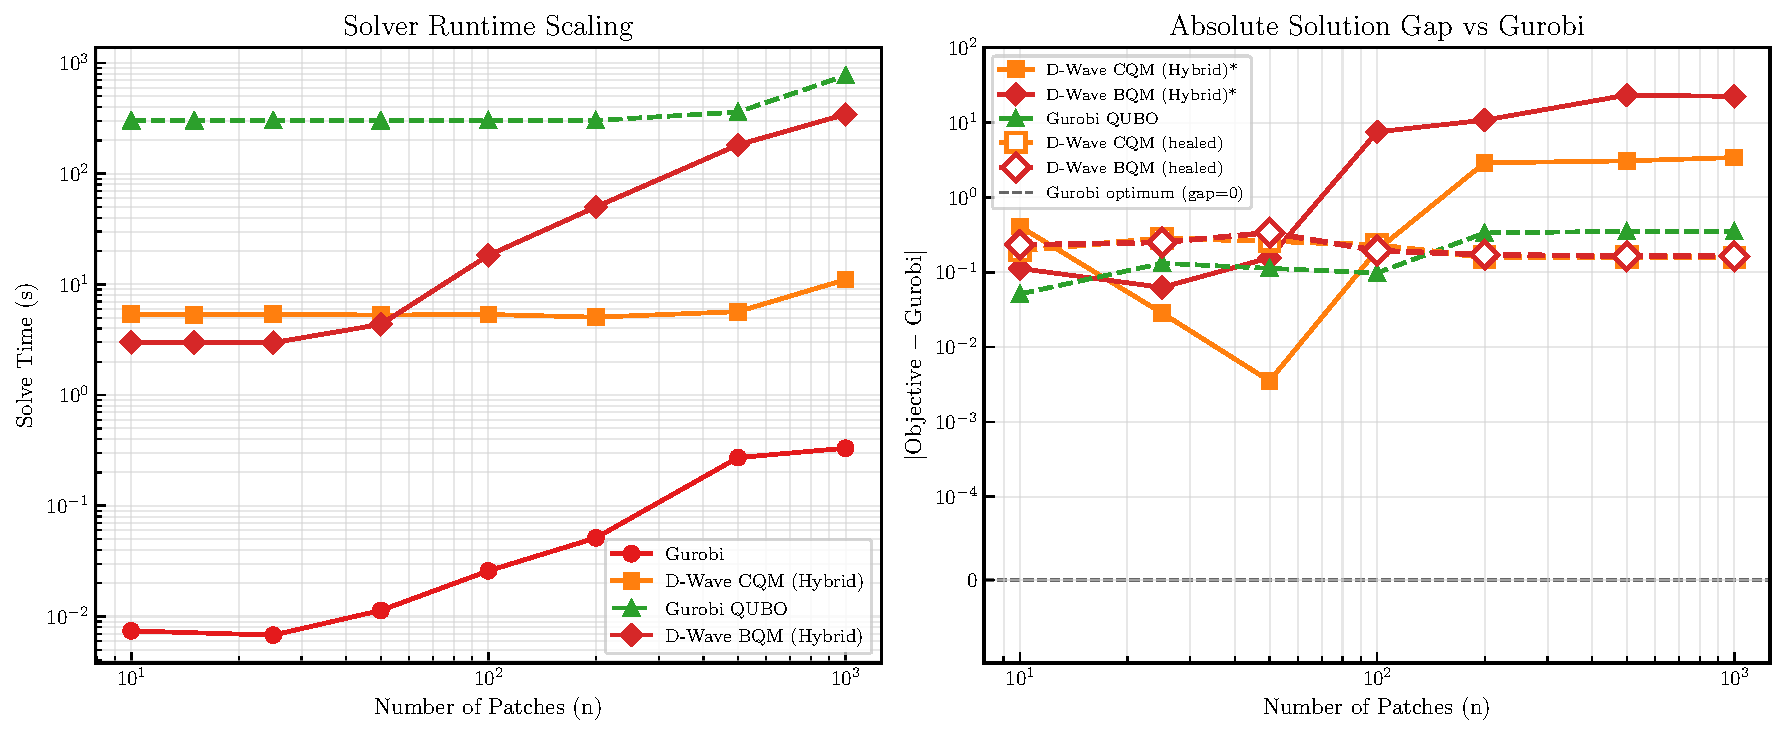
\includegraphics[width=\textwidth]{@todo/report/images/Plots/study1_hybrid_performance.pdf}
\caption{%
\textbf{Study~1: Hybrid solver benchmark (10--1{,}000 patches).}
\emph{Left panel (Solver Runtime Scaling):} Wall-clock solve time on log--log axes.
Gurobi on the native CQM formulation (red circles) scales from 0.006\,s at $n{=}10$ to 3.8\,s at $n{=}10{,}000$, remaining the fastest solver at every scale.
The D-Wave CQM hybrid solver (orange squares) maintains a near-constant ${\sim}$5\,s runtime up to $n{=}500$, increasing to 11\,s at $n{=}1{,}000$---dominated by classical orchestration, with actual QPU annealing constituting only 0.3--1.3\% of wall time.
Gurobi on the penalty-encoded QUBO (green triangles, dashed)
consistently hits its 300\,s timeout regardless of scale, confirming that penalty encoding destroys the branch-and-bound exploitable structure.
The D-Wave BQM hybrid solver (red diamonds) handles the penalty-encoded form but exhibits steep scaling: 3.0\,s at $n{=}10$ to 344\,s at $n{=}1{,}000$.
\emph{Right panel (Absolute Solution Gap vs Gurobi):} The absolute gap
$|Z_{\text{solver}} - Z^{\star}_{\text{Gurobi}}|$ on a symmetric-log scale.
Solid markers are raw objectives; open markers with dashed lines show healed (feasibility-repaired) objectives.
The D-Wave CQM solver achieves gaps below $10^{-2}$ at $n{=}25$--$50$ (near-optimal after healing), but infeasible raw objectives at $n{\geq}200$ inflate the raw gap to 2.9--3.4.
The D-Wave BQM solver exhibits a raw gap exceeding 10 at $n{\geq}200$ due to severe one-hot violations.
Gurobi QUBO---despite timing out---produces feasible solutions with a moderate gap of 0.05--0.33, smaller than the major infeasibility-driven inflation of D-Wave solvers at large scales.
A healed-objective analysis (\cref{sec:healing}) narrows the CQM gap to ${\sim}0.1$--$0.2$ at scale, but the BQM gap remains above 0.1 everywhere.
Overall, Gurobi on the native CQM formulation dominates in both speed and solution quality.}
\label{fig:hybrid_solver_performance}
\end{figure*}

% ── Study 1 Violation Table ───────────────────────────────────────────────────
\begin{table}[t]
\centering
\caption{Hybrid solver constraint violations (Study~1).
CQM produces 12 violations at $n{=}15$ and 2 at $n{=}25$; BQM produces 9--11 violations at $n{\leq}25$ (all one-crop-per-patch type).
Both solvers become feasible at $n{\geq}50$.}
\label{tab:study1_violations}
\footnotesize
\resizebox{\columnwidth}{!}{%
\begin{tabular}{rrrcrc}
\toprule
\textbf{Patches} & \textbf{CQM Viols} & \textbf{CQM Feasible} & \textbf{BQM Viols} & \textbf{BQM Feasible} \\
\midrule
10    & 0  & Yes & 9  & No  \\
15    & 12 & No  & 10 & No  \\
25    & 2  & No  & 11 & No  \\
50    & 0  & Yes & 0  & Yes \\
100   & 0  & Yes & 0  & Yes \\
200   & 0  & Yes & 0  & Yes \\
500   & 0  & Yes & 0  & Yes \\
1{,}000 & 0  & Yes & 0  & Yes \\
\bottomrule
\end{tabular}
}
\end{table}


\subsection{QPU Decomposition and the Embedding Bottleneck}
\label{subsec:qpu}

Table~\ref{tab:qpu_scaling} isolates QPU annealing time from classical embedding time for Multilevel(10) decomposition.
QPU time follows $T_{\text{QPU}} \approx k \cdot n_{\text{part}} \cdot t_{\text{anneal}}$, where $k{=}1$--$3$ coordination rounds, $n_{\text{part}}$ grows linearly with plot count, and $t_{\text{anneal}}{\approx}100$\,ms per partition including QPU access latency~\cite{pelofske2021parallel, marshall2019power}.
QPU annealing therefore scales linearly and remains below 27\,s at 1{,}000~plots.
Classical MinorMiner embedding grows from 10.2\,s to 1{,}309\,s over the same range, constituting \textbf{95--99\%} of total runtime at every scale.
This is the central finding: \emph{classical embedding, not quantum sampling, is the binding bottleneck}.

\begin{table}[t]
\centering
\caption{QPU time vs.\ classical embedding time for Multilevel(10) decomposition. Embedding constitutes 76--80\% of total time; QPU remains 1.2--3.1\% across all scales.}
\label{tab:qpu_scaling}
\footnotesize
\resizebox{\columnwidth}{!}{%
\begin{tabular}{rrrrrr}
\toprule
\textbf{Farms} & \textbf{Total (s)} & \textbf{QPU (s)} & \textbf{Embed (s)} & \textbf{QPU\%} & \textbf{Embed\%} \\
\midrule
10      &    13.5 &  0.42 &    10.2 &  3.1\% & 75.7\% \\
50      &   128.6 &  1.51 &   110.2 &  1.2\% & 85.7\% \\
100     &   175.1 &  2.83 &   144.6 &  1.6\% & 82.6\% \\
200     &   388.7 &  5.48 &   315.3 &  1.4\% & 81.1\% \\
500     &   839.1 & 13.44 &   677.8 &  1.6\% & 80.8\% \\
1{,}000 & 1{,}632.7 & 26.83 & 1{,}308.9 &  1.6\% & 80.2\% \\
\bottomrule
\end{tabular}
}
\end{table}

Table~\ref{tab:quality_1000} compares solution quality across all methods at the 1{,}000-farm scale.
Direct QPU embedding fails entirely, confirming that decomposition is mandatory for practical problem sizes.
Among the full-span methods, HybridGrid(5,9) achieves the best balance: a gap of 0.043 with zero constraint violations in 845\,s.
Coordinated decomposition reaches the lowest raw gap (0.137) but accumulates 23 one-hot violations---and its healed objective drops to $-0.038$, indicating that the apparent objective advantage is substantially driven by infeasible multi-crop assignments.
Multilevel(10), with a gap of 0.171 and zero violations at 1{,}000 farms, offers reliable decomposition quality albeit with larger objective loss.
CQM-First shows variable performance: a gap of 0.171 at 1{,}000 farms with zero violations, but its healed objective of $-0.034$ reveals that at this scale the repaired solution is slightly worse than a trivial all-idle allocation.

\begin{table}[t]
\centering
\caption{Solution quality at the 1{,}000-farm scale. Gap = $|Z_{\text{method}} - Z^{\star}_{\text{Gurobi}}|$. ``(h)'' rows show healed objectives where violations exist. HybridGrid(5,9) achieves the smallest gap among violation-free QPU methods. Gurobi decomposed methods (marked *) use a stricter formulation; CQMFirst* has 3 food-group violations; all others incur 5.}
\label{tab:quality_1000}
\footnotesize
\resizebox{\columnwidth}{!}{%
\begin{tabular}{lcccc}
\toprule
\textbf{Method} & \textbf{Obj.} & \textbf{Gap} & \textbf{Viol.} & \textbf{Time\,(s)} \\
\midrule
Gurobi GT (optimal)             & 0.429 & 0.000 &  0 &     0.3 \\
\midrule
HybridGrid(5,9) \emph{QPU}      & 0.386 & 0.043 &  0 &   845.4 \\
Multilevel(10) \emph{QPU}       & 0.258 & 0.171 &  0 & 1{,}632.7 \\
CQM-First \emph{QPU}            & 0.258 & 0.171 &  0 & 3{,}495.4 \\
Coordinated \emph{QPU}          & 0.293 & 0.137 & 23 & 3{,}058.0 \\
Coordinated \emph{QPU} (h)      & $-$0.038 & 0.467 & — &         \\
\midrule
Gurobi [HybridGrid(5,9)]*       & 1.011 & 0.582 &  5 &     0.5 \\
Gurobi [HybridGrid(5,9)]* (h)   & 0.428 & 0.001 & — &         \\
Gurobi [Multilevel(10)]*        & 0.430 & 0.001 &  5 &     0.2 \\
Gurobi [Multilevel(10)]* (h)    & 0.428 & 0.001 & — &         \\
Gurobi [CQMFirst]*              & 0.353 & 0.076 &  3 &    $<$0.1 \\
Gurobi [CQMFirst]* (h)          & 0.352 & 0.077 & — &         \\
Gurobi [Coordinated]*           & 0.430 & 0.001 &  5 &    $<$0.1 \\
Gurobi [Coordinated]* (h)       & 0.428 & 0.001 & — &         \\
\bottomrule
\end{tabular}
}
\end{table}

\noindent
\textbf{Gurobi decomposed baselines.}
To disentangle decomposition quality from QPU approximation, we also solve each decomposed subproblem exactly with Gurobi (marked * in tables and plots) for all four full-span decomposition strategies: HybridGrid(5,9), Multilevel(10), CQM-First, and Coordinated.
These Gurobi decomposed variants use a stricter constraint formulation (Variant-A).
Multilevel(10)* and Coordinated* consistently incur exactly 5 food-group violations regardless of scale---a structural artefact of the decomposition breaking global coverage constraints.
CQMFirst* incurs 3 food-group violations, and HybridGrid(5,9)* also incurs 5.
At the Multilevel and Coordinated granularity, Gurobi recovers near-optimal objectives within each subproblem (healed gap ${\sim}10^{-3}$), demonstrating that the decomposition itself preserves solution quality well.
CQMFirst* achieves a lower raw objective (${\sim}0.353$ vs ${\sim}0.429$), reflecting that the U-master step pre-selects foods before patch assignment, producing a slightly different feasible solution.
HybridGrid(5,9)* exhibits a larger raw objective ($1.011$) because its coarser grid partitioning produces solutions with inflated benefit from infeasible cross-boundary assignments; after healing, its gap drops to ${\sim}10^{-4}$.
This comparison confirms that much of the gap in QPU results originates from the decomposition and embedding pipeline rather than from QPU sampling quality.

\Cref{fig:qpu_comprehensive} presents the full comprehensive benchmark.

\begin{figure*}[t]
\centering
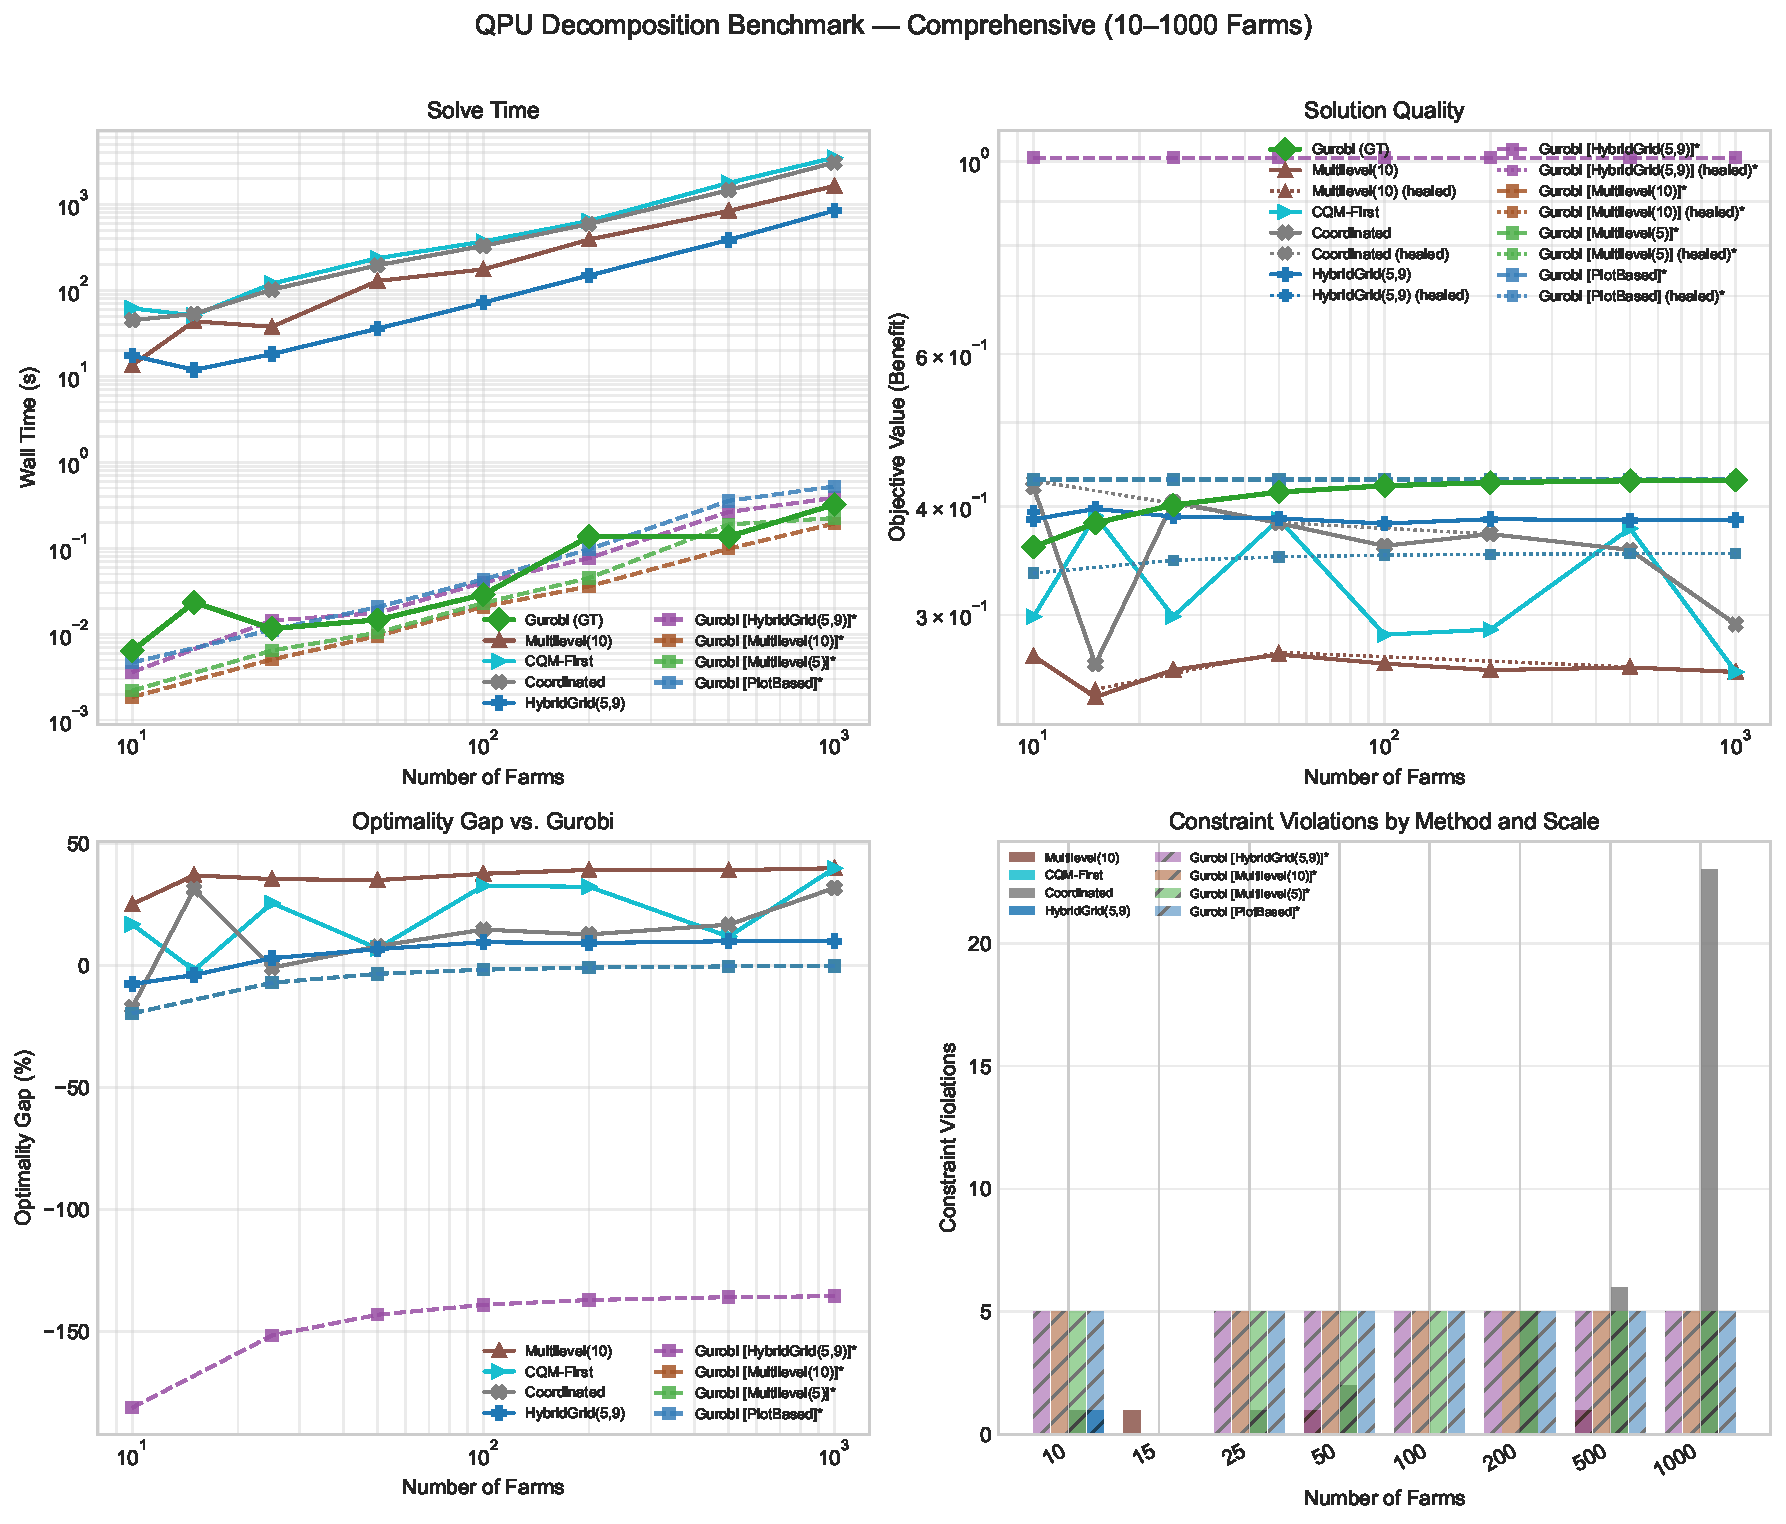
\includegraphics[width=\textwidth]{@todo/report/images/Plots/qpu_benchmark_comprehensive.pdf}
\caption{%
\textbf{Study~2: QPU decomposition benchmark---comprehensive view (10--1{,}000 farms).}
All four full-span QPU methods are shown alongside their corresponding Gurobi decomposed baselines (dashed lines, marked~*): HybridGrid(5,9), Multilevel(10), CQM-First, and Coordinated.
Gurobi decomposed baselines solve the same partitioned subproblems exactly to isolate QPU approximation error from decomposition quality loss.
\emph{Left panel (Solve Time):} Wall-clock time on log--log axes.
Gurobi on the full (undivided) problem (green diamonds) scales from 0.007\,s to 0.27\,s---three to four orders of magnitude faster than any decomposition workflow.
HybridGrid(5,9) (blue pentagons) is the fastest QPU method, scaling from 17\,s to 845\,s, with actual QPU time comprising 6--15\% of wall time (the remainder being classical embedding at 18--28\% and orchestration overhead).
Multilevel(10) (brown triangles) and CQM-First (cyan chevrons) scale more steeply (1{,}633\,s and 3{,}495\,s at $n{=}1{,}000$ respectively), with embedding dominating at 80+\% of runtime.
Coordinated (grey Xs) tracks CQM-First closely (3{,}058\,s at $n{=}1{,}000$).
All four Gurobi decomposed baselines (dashed lines) complete in $<$10\,s at every tested scale, confirming that decomposition overhead is negligible without embedding.
\emph{Right panel (Absolute Solution Gap vs Gurobi):} The absolute objective gap
$|Z - Z^{\star}|$ on a symmetric-log scale.
HybridGrid(5,9) (blue, solid) maintains the tightest gap among QPU methods, ranging from 0.027 at $n{=}10$ to 0.043 at $n{=}1{,}000$, with zero constraint violations across all scales.
Multilevel(10) (brown, solid) exhibits a gap of 0.09--0.17, increasing modestly with scale.
CQM-First (cyan) shows inconsistent performance: gaps range from 0.007 to 0.17 depending on scale.
Coordinated (grey) achieves raw gaps of 0.003--0.14 but incurs 1--23 one-hot violations; its healed gap (dotted grey) rises substantially at small scales, indicating that the apparent objective advantage largely reflects infeasible multi-crop assignments.
Among the Gurobi decomposed baselines, Multilevel(10) and Coordinated* recover near-optimal objectives (gap ${\sim}10^{-3}$ after healing); HybridGrid(5,9)* shows a fixed raw gap of ${\sim}0.58$ (inflated by 5 persistent food-group violations; healed gap ${\sim}10^{-4}$); CQMFirst* incurs 3 food-group violations with a raw gap of ${\sim}0.076$ and healed gap ${\sim}0.077$.
The dashed lines serve as a ceiling: the gap between a QPU method and its Gurobi decomposed counterpart isolates QPU-attributable approximation error.
For HybridGrid(5,9), this QPU-attributable gap is 0.01--0.04; for Multilevel(10) it is 0.09--0.17.
Overall, no QPU method matches the Gurobi optimum, but HybridGrid(5,9) consistently achieves $\leq$10\% relative gap with full feasibility.
}
\label{fig:qpu_comprehensive}
\end{figure*}

Table~\ref{tab:violations} breaks down constraint violations by decomposition strategy across all tested scales (full data for all 8~methods).
Two violation patterns emerge: \emph{food-group violations} arise when partition boundaries prevent global category constraints from being satisfied, and \emph{one-hot violations} arise when coordination rounding assigns zero or multiple crops to a single plot.

\begin{table}[t]
\centering
\caption{Constraint violation summary by decomposition strategy (full-span methods).
Coordinated is the only QPU method with one-hot violations, escalating to 23 at $n{=}1{,}000$ (38 total across all scales).
HybridGrid(5,9) has a single food-group violation at $n{=}10$ only.}
\label{tab:violations}
\footnotesize
\setlength{\tabcolsep}{3pt}
\resizebox{\columnwidth}{!}{%
\begin{tabular}{lcccc}
\toprule
\textbf{Method} & \textbf{Entries w/\,Viol.} & \textbf{Total} & \textbf{Rate} & \textbf{Type} \\
\midrule
CQM-First           & 0/8 (0\%)  &  0 & None & --- \\
Louvain             & 1/5 (20\%) &  1 & Low  & Food group \\
HybridGrid(5,9)     & 1/8 (12\%) &  1 & Low  & Food group \\
Multilevel(10)      & 3/8 (38\%) &  3 & Med. & Food group \\
Multilevel(5)       & 3/5 (60\%) &  4 & Med. & Food group \\
PlotBased           & 2/5 (40\%) &  2 & Med. & Food group \\
Spectral(10)        & 3/5 (60\%) &  3 & Med. & Food group \\
Coordinated         & 6/8 (75\%) & 38 & High & One-hot \\
\bottomrule
\end{tabular}
}
\end{table}

% ── Post-hoc feasibility repair ──────────────────────────────────────────────
% AUTO-GENERATED section — do not edit manually
% Place inside the relevant results section, e.g.:
%   % AUTO-GENERATED section — do not edit manually
% Place inside the relevant results section, e.g.:
%   % AUTO-GENERATED section — do not edit manually
% Place inside the relevant results section, e.g.:
%   \input{sections/healing_procedure}

\subsection{Post-Hoc Feasibility Repair and Healed Objective}
\label{sec:healing}

Several solvers — D-Wave BQM, D-Wave CQM, and the Gurobi decomposed variants —
return solutions that are \emph{infeasible} with respect to one or more
constraints.
To provide a meaningful quality comparison on a common, feasible baseline, we
apply a greedy, \emph{one-shot} repair procedure per solution and report the
resulting \emph{healed objective} alongside (or in place of) the raw objective.
The healed objective is always $\leq$ the raw objective, so it is a
\emph{lower-bound} on the true feasible value the solver would have obtained had
it found a feasible solution.

% -----------------------------------------------------------------------
\subsubsection{Violation Types}
\label{sec:healing:violtypes}

\paragraph{Study~1 (patch benchmark, BQM/CQM).}
The patch-level QUBO/CQM formulation enforces an \emph{at-most-one-crop-per-patch}
constraint.
All observed violations are of this single type: the solver assigns two crops
$c_1, c_2$ to the same patch $p$ (both indicator variables $Y_{p,c_1}$ and
$Y_{p,c_2}$ are set to 1).

\paragraph{Study~2 and Gurobi decomposed (farm benchmark).}
Two constraint types are violated:
\begin{enumerate}
  \item \textbf{One-crop-per-farm} ($\sum_c Y_{f,c} \leq 1$): analogous to the
        patch case — multiple crops are assigned to a single farm.
  \item \textbf{Food-group coverage} ($\sum_{f} Y_{f,c} \geq 1$ for each food
        group): at least one farm must be assigned to a representative crop of a
        specified food group; the solver fails to satisfy one or more of these
        coverage requirements.
\end{enumerate}

% -----------------------------------------------------------------------
\subsubsection{Repair for One-Crop-per-Patch/Farm Violations}
\label{sec:healing:onecrop}

Let $n$ denote the total number of patches (farms), $A_{\text{tot}}$ the total
cultivable area, and $A_p = A_{\text{tot}} / n$ the uniform area per patch
(farm).
Define the normalised per-crop contribution on a violating patch/farm as
\begin{equation}
  \delta_{p,c} \;=\; b_c \cdot \frac{A_p}{A_{\text{tot}}} ,
  \label{eq:patch_contrib}
\end{equation}
where $b_c \geq 0$ is the benefit coefficient of crop $c$ (from the
rotation-benefit matrix).

For each violating patch/farm $p$ with assigned crops $\mathcal{C}_p$
($|\mathcal{C}_p| \geq 2$), we \textbf{remove the minimum-benefit crop}:
\begin{equation}
  \text{gain}_p \;=\; \min_{c\,\in\,\mathcal{C}_p}\; \delta_{p,c} .
  \label{eq:onecrop_gain}
\end{equation}
The healed objective is then
\begin{equation}
  \tilde{f} \;=\; f_{\text{raw}} - \sum_{p \in \mathcal{V}} \text{gain}_p ,
  \label{eq:healed_onecrop}
\end{equation}
where $\mathcal{V}$ is the set of violating patches/farms.
This repair is exact: removing one crop from patch $p$ leaves exactly one
assigned crop, fully restoring feasibility for that patch.

For the \textbf{Gurobi decomposed} variants,
$\tilde{f}$ is pre-computed by the benchmark script and stored as
\texttt{healed\_objective} in
\texttt{solver\_comparison\_results\_hard.json}.  The repair is performed
analytically during the benchmark run using the same procedure above.

For the \textbf{D-Wave BQM/CQM} (Study~1), the repair is applied
post-hoc from the stored \texttt{solution\_plantations} dictionary
$\{Y_{p,c}\}$ by identifying $\mathcal{C}_p = \{c : Y_{p,c} \geq 0.5\}$ for
each violating patch and applying \cref{eq:healed_onecrop}.

% -----------------------------------------------------------------------
\subsubsection{Repair for Food-Group Coverage Violations}
\label{sec:healing:foodgroup}

A food-group constraint of the form
$\sum_{f} Y_{f,g} \geq g_{\min}$
is violated when the number of farms planting a crop from group $g$ falls short
by $\Delta_g = g_{\min} - \sum_f Y_{f,g} > 0$ farms.

The repair swaps $\Delta_g$ existing farm assignments to a representative crop
of group $g$.  We assume the representative crop has benefit $b_g \approx 0$
(starchy-staple crops, which constitute the majority of violated food groups),
so the swap cost equals the full contribution of the farm that is re-assigned.
We choose the \textbf{minimum-benefit farm} to swap, minimising the objective
loss:
\begin{equation}
  \text{gain}_g \;=\; \Delta_g \cdot
    \min_{f\,\in\,\mathcal{F}_{\text{active}}} \;
    \sum_{c\,\in\,\mathcal{C}_f} b_c \cdot \frac{A_f}{A_{\text{tot}}} ,
  \label{eq:foodgroup_gain}
\end{equation}
where $\mathcal{F}_{\text{active}}$ is the set of farms not already assigned to
group $g$.
The total healed objective when both violation types are present is
\begin{equation}
  \tilde{f} \;=\; f_{\text{raw}}
    - \sum_{p\,\in\,\mathcal{V}} \text{gain}_p
    - \sum_{g\,\in\,\mathcal{G}} \text{gain}_g .
  \label{eq:healed_full}
\end{equation}

% -----------------------------------------------------------------------
\subsubsection{Interpretation}
\label{sec:healing:interp}

The healed objective $\tilde{f}$ provides a pessimistic (lower-bound) estimate
of the feasible solution quality.
A large gap $f_{\text{raw}} - \tilde{f}$ signals that the solver's objective
inflation is substantially driven by constraint violations: the reported
$f_{\text{raw}}$ is not a valid crop-allocation benefit.
Conversely, a small gap — as observed for most QPU methods and all Gurobi
decomposed variants beyond $n = 25$ farms — indicates that the solution is
\emph{nearly} feasible and only minor repairs are needed.

In the figures, raw objectives are shown as solid lines and healed objectives
as dotted lines of matching colour.  Scales at which raw and healed coincide
(no violations) are omitted from the dotted series.


\subsection{Post-Hoc Feasibility Repair and Healed Objective}
\label{sec:healing}

Several solvers — D-Wave BQM, D-Wave CQM, and the Gurobi decomposed variants —
return solutions that are \emph{infeasible} with respect to one or more
constraints.
To provide a meaningful quality comparison on a common, feasible baseline, we
apply a greedy, \emph{one-shot} repair procedure per solution and report the
resulting \emph{healed objective} alongside (or in place of) the raw objective.
The healed objective is always $\leq$ the raw objective, so it is a
\emph{lower-bound} on the true feasible value the solver would have obtained had
it found a feasible solution.

% -----------------------------------------------------------------------
\subsubsection{Violation Types}
\label{sec:healing:violtypes}

\paragraph{Study~1 (patch benchmark, BQM/CQM).}
The patch-level QUBO/CQM formulation enforces an \emph{at-most-one-crop-per-patch}
constraint.
All observed violations are of this single type: the solver assigns two crops
$c_1, c_2$ to the same patch $p$ (both indicator variables $Y_{p,c_1}$ and
$Y_{p,c_2}$ are set to 1).

\paragraph{Study~2 and Gurobi decomposed (farm benchmark).}
Two constraint types are violated:
\begin{enumerate}
  \item \textbf{One-crop-per-farm} ($\sum_c Y_{f,c} \leq 1$): analogous to the
        patch case — multiple crops are assigned to a single farm.
  \item \textbf{Food-group coverage} ($\sum_{f} Y_{f,c} \geq 1$ for each food
        group): at least one farm must be assigned to a representative crop of a
        specified food group; the solver fails to satisfy one or more of these
        coverage requirements.
\end{enumerate}

% -----------------------------------------------------------------------
\subsubsection{Repair for One-Crop-per-Patch/Farm Violations}
\label{sec:healing:onecrop}

Let $n$ denote the total number of patches (farms), $A_{\text{tot}}$ the total
cultivable area, and $A_p = A_{\text{tot}} / n$ the uniform area per patch
(farm).
Define the normalised per-crop contribution on a violating patch/farm as
\begin{equation}
  \delta_{p,c} \;=\; b_c \cdot \frac{A_p}{A_{\text{tot}}} ,
  \label{eq:patch_contrib}
\end{equation}
where $b_c \geq 0$ is the benefit coefficient of crop $c$ (from the
rotation-benefit matrix).

For each violating patch/farm $p$ with assigned crops $\mathcal{C}_p$
($|\mathcal{C}_p| \geq 2$), we \textbf{remove the minimum-benefit crop}:
\begin{equation}
  \text{gain}_p \;=\; \min_{c\,\in\,\mathcal{C}_p}\; \delta_{p,c} .
  \label{eq:onecrop_gain}
\end{equation}
The healed objective is then
\begin{equation}
  \tilde{f} \;=\; f_{\text{raw}} - \sum_{p \in \mathcal{V}} \text{gain}_p ,
  \label{eq:healed_onecrop}
\end{equation}
where $\mathcal{V}$ is the set of violating patches/farms.
This repair is exact: removing one crop from patch $p$ leaves exactly one
assigned crop, fully restoring feasibility for that patch.

For the \textbf{Gurobi decomposed} variants,
$\tilde{f}$ is pre-computed by the benchmark script and stored as
\texttt{healed\_objective} in
\texttt{solver\_comparison\_results\_hard.json}.  The repair is performed
analytically during the benchmark run using the same procedure above.

For the \textbf{D-Wave BQM/CQM} (Study~1), the repair is applied
post-hoc from the stored \texttt{solution\_plantations} dictionary
$\{Y_{p,c}\}$ by identifying $\mathcal{C}_p = \{c : Y_{p,c} \geq 0.5\}$ for
each violating patch and applying \cref{eq:healed_onecrop}.

% -----------------------------------------------------------------------
\subsubsection{Repair for Food-Group Coverage Violations}
\label{sec:healing:foodgroup}

A food-group constraint of the form
$\sum_{f} Y_{f,g} \geq g_{\min}$
is violated when the number of farms planting a crop from group $g$ falls short
by $\Delta_g = g_{\min} - \sum_f Y_{f,g} > 0$ farms.

The repair swaps $\Delta_g$ existing farm assignments to a representative crop
of group $g$.  We assume the representative crop has benefit $b_g \approx 0$
(starchy-staple crops, which constitute the majority of violated food groups),
so the swap cost equals the full contribution of the farm that is re-assigned.
We choose the \textbf{minimum-benefit farm} to swap, minimising the objective
loss:
\begin{equation}
  \text{gain}_g \;=\; \Delta_g \cdot
    \min_{f\,\in\,\mathcal{F}_{\text{active}}} \;
    \sum_{c\,\in\,\mathcal{C}_f} b_c \cdot \frac{A_f}{A_{\text{tot}}} ,
  \label{eq:foodgroup_gain}
\end{equation}
where $\mathcal{F}_{\text{active}}$ is the set of farms not already assigned to
group $g$.
The total healed objective when both violation types are present is
\begin{equation}
  \tilde{f} \;=\; f_{\text{raw}}
    - \sum_{p\,\in\,\mathcal{V}} \text{gain}_p
    - \sum_{g\,\in\,\mathcal{G}} \text{gain}_g .
  \label{eq:healed_full}
\end{equation}

% -----------------------------------------------------------------------
\subsubsection{Interpretation}
\label{sec:healing:interp}

The healed objective $\tilde{f}$ provides a pessimistic (lower-bound) estimate
of the feasible solution quality.
A large gap $f_{\text{raw}} - \tilde{f}$ signals that the solver's objective
inflation is substantially driven by constraint violations: the reported
$f_{\text{raw}}$ is not a valid crop-allocation benefit.
Conversely, a small gap — as observed for most QPU methods and all Gurobi
decomposed variants beyond $n = 25$ farms — indicates that the solution is
\emph{nearly} feasible and only minor repairs are needed.

In the figures, raw objectives are shown as solid lines and healed objectives
as dotted lines of matching colour.  Scales at which raw and healed coincide
(no violations) are omitted from the dotted series.


\subsection{Post-Hoc Feasibility Repair and Healed Objective}
\label{sec:healing}

Several solvers — D-Wave BQM, D-Wave CQM, and the Gurobi decomposed variants —
return solutions that are \emph{infeasible} with respect to one or more
constraints.
To provide a meaningful quality comparison on a common, feasible baseline, we
apply a greedy, \emph{one-shot} repair procedure per solution and report the
resulting \emph{healed objective} alongside (or in place of) the raw objective.
The healed objective is always $\leq$ the raw objective, so it is a
\emph{lower-bound} on the true feasible value the solver would have obtained had
it found a feasible solution.

% -----------------------------------------------------------------------
\subsubsection{Violation Types}
\label{sec:healing:violtypes}

\paragraph{Study~1 (patch benchmark, BQM/CQM).}
The patch-level QUBO/CQM formulation enforces an \emph{at-most-one-crop-per-patch}
constraint.
All observed violations are of this single type: the solver assigns two crops
$c_1, c_2$ to the same patch $p$ (both indicator variables $Y_{p,c_1}$ and
$Y_{p,c_2}$ are set to 1).

\paragraph{Study~2 and Gurobi decomposed (farm benchmark).}
Two constraint types are violated:
\begin{enumerate}
  \item \textbf{One-crop-per-farm} ($\sum_c Y_{f,c} \leq 1$): analogous to the
        patch case — multiple crops are assigned to a single farm.
  \item \textbf{Food-group coverage} ($\sum_{f} Y_{f,c} \geq 1$ for each food
        group): at least one farm must be assigned to a representative crop of a
        specified food group; the solver fails to satisfy one or more of these
        coverage requirements.
\end{enumerate}

% -----------------------------------------------------------------------
\subsubsection{Repair for One-Crop-per-Patch/Farm Violations}
\label{sec:healing:onecrop}

Let $n$ denote the total number of patches (farms), $A_{\text{tot}}$ the total
cultivable area, and $A_p = A_{\text{tot}} / n$ the uniform area per patch
(farm).
Define the normalised per-crop contribution on a violating patch/farm as
\begin{equation}
  \delta_{p,c} \;=\; b_c \cdot \frac{A_p}{A_{\text{tot}}} ,
  \label{eq:patch_contrib}
\end{equation}
where $b_c \geq 0$ is the benefit coefficient of crop $c$ (from the
rotation-benefit matrix).

For each violating patch/farm $p$ with assigned crops $\mathcal{C}_p$
($|\mathcal{C}_p| \geq 2$), we \textbf{remove the minimum-benefit crop}:
\begin{equation}
  \text{gain}_p \;=\; \min_{c\,\in\,\mathcal{C}_p}\; \delta_{p,c} .
  \label{eq:onecrop_gain}
\end{equation}
The healed objective is then
\begin{equation}
  \tilde{f} \;=\; f_{\text{raw}} - \sum_{p \in \mathcal{V}} \text{gain}_p ,
  \label{eq:healed_onecrop}
\end{equation}
where $\mathcal{V}$ is the set of violating patches/farms.
This repair is exact: removing one crop from patch $p$ leaves exactly one
assigned crop, fully restoring feasibility for that patch.

For the \textbf{Gurobi decomposed} variants,
$\tilde{f}$ is pre-computed by the benchmark script and stored as
\texttt{healed\_objective} in
\texttt{solver\_comparison\_results\_hard.json}.  The repair is performed
analytically during the benchmark run using the same procedure above.

For the \textbf{D-Wave BQM/CQM} (Study~1), the repair is applied
post-hoc from the stored \texttt{solution\_plantations} dictionary
$\{Y_{p,c}\}$ by identifying $\mathcal{C}_p = \{c : Y_{p,c} \geq 0.5\}$ for
each violating patch and applying \cref{eq:healed_onecrop}.

% -----------------------------------------------------------------------
\subsubsection{Repair for Food-Group Coverage Violations}
\label{sec:healing:foodgroup}

A food-group constraint of the form
$\sum_{f} Y_{f,g} \geq g_{\min}$
is violated when the number of farms planting a crop from group $g$ falls short
by $\Delta_g = g_{\min} - \sum_f Y_{f,g} > 0$ farms.

The repair swaps $\Delta_g$ existing farm assignments to a representative crop
of group $g$.  We assume the representative crop has benefit $b_g \approx 0$
(starchy-staple crops, which constitute the majority of violated food groups),
so the swap cost equals the full contribution of the farm that is re-assigned.
We choose the \textbf{minimum-benefit farm} to swap, minimising the objective
loss:
\begin{equation}
  \text{gain}_g \;=\; \Delta_g \cdot
    \min_{f\,\in\,\mathcal{F}_{\text{active}}} \;
    \sum_{c\,\in\,\mathcal{C}_f} b_c \cdot \frac{A_f}{A_{\text{tot}}} ,
  \label{eq:foodgroup_gain}
\end{equation}
where $\mathcal{F}_{\text{active}}$ is the set of farms not already assigned to
group $g$.
The total healed objective when both violation types are present is
\begin{equation}
  \tilde{f} \;=\; f_{\text{raw}}
    - \sum_{p\,\in\,\mathcal{V}} \text{gain}_p
    - \sum_{g\,\in\,\mathcal{G}} \text{gain}_g .
  \label{eq:healed_full}
\end{equation}

% -----------------------------------------------------------------------
\subsubsection{Interpretation}
\label{sec:healing:interp}

The healed objective $\tilde{f}$ provides a pessimistic (lower-bound) estimate
of the feasible solution quality.
A large gap $f_{\text{raw}} - \tilde{f}$ signals that the solver's objective
inflation is substantially driven by constraint violations: the reported
$f_{\text{raw}}$ is not a valid crop-allocation benefit.
Conversely, a small gap — as observed for most QPU methods and all Gurobi
decomposed variants beyond $n = 25$ farms — indicates that the solution is
\emph{nearly} feasible and only minor repairs are needed.

In the figures, raw objectives are shown as solid lines and healed objectives
as dotted lines of matching colour.  Scales at which raw and healed coincide
(no violations) are omitted from the dotted series.


\section{Discussion \& Conclusion}
\label{sec:DiscussionConclusion}

This paper reported two complementary experiments---a hybrid solver benchmark and a transparent QPU decomposition study---that characterise where computational effort concentrates when mapping a structured agricultural allocation problem onto quantum annealing hardware.
Three engineering lessons emerge.

\textbf{Penalty encoding breaks classical solvers but not D-Wave.}
The BP formulation is tractable when submitted via D-Wave's CQM format, which preserves explicit constraints: Gurobi solves instances optimally in 0.007--0.27\,s across 10--1{,}000~plots, while D-Wave's CQM hybrid solver returns solutions in ${\sim}$5--11\,s.
Converting those constraints into QUBO penalty terms---as required for direct QPU execution---renders Gurobi ineffective at every tested scale (300+\,s timeouts with objective degradation to $Z{=}0$ above 500~patches), whereas D-Wave's BQM hybrid solver still completes in 3--344\,s.
This is a structural consequence of destroying algebraic constraint information, not a solver deficiency~\cite{wolsey1998integer, barahona1982computational}.
QA's energy-minimisation paradigm is unaffected, providing practical motivation for the quantum workflow even where decomposition is necessary.

\textbf{Hybrid solvers are predominantly classical---and Gurobi still wins.}
QPU time constitutes 0.3--1.3\% of D-Wave CQM wall-clock time and 1.7--3.5\% of BQM time; the remainder is classical orchestration~\cite{dwave:solver_properties_all}.
More critically, the D-Wave solvers produce infeasible solutions at several scales: CQM violates one-hot constraints at $n{=}15$--25 and reports inflated objectives ($Z{>}3.0$) at $n{\geq}200$, while BQM produces 9--11 violations at small scales and $Z{>}22$ at $n{=}500$.
After feasibility repair (healing), the CQM gap to Gurobi is ${\sim}0.1$--$0.2$, and BQM exceeds 0.1 everywhere.
Gurobi on the native CQM formulation dominates on every metric---speed, optimality, and feasibility---underscoring that hybrid solvers, despite handling penalty encoding, do not yet offer a competitive advantage for this problem class.

\textbf{QPU annealing scales well; embedding does not.}
Annealing time grows linearly with partition count and stays below 27\,s at 1{,}000~farms (1.6\% of total time for Multilevel(10)).
Classical MinorMiner embedding grows from 10\,s to 1{,}309\,s over the same range, constituting 76--81\% of total runtime.
Among the QPU decomposition strategies, HybridGrid(5,9) achieves the best quality--speed trade-off: absolute objective gap of 0.027--0.043 with zero violations across all scales above $n{=}10$, and the shortest wall times (17--845\,s).
Multilevel(10) and CQM-First offer zero-violation solutions but with larger gaps (${\sim}$0.17);
Coordinated reaches lower raw gaps but at the cost of escalating one-hot violations (23 at $n{=}1{,}000$), making its raw objectives unreliable.

\textbf{Decomposition, not QPU, is the main quality bottleneck.}
Solving decomposed subproblems exactly with Gurobi (decomposed baselines) recovers near-optimal objectives for most partition strategies---e.g.\ Multilevel(10) under Gurobi yields gap ${\sim}10^{-3}$ after healing, versus 0.171 under QPU.
The QPU-attributable gap for HybridGrid(5,9) is only 0.01--0.04, indicating that the QPU samples are high-quality within each subproblem.
The dominant quality loss therefore originates from decomposition boundary effects and global constraint propagation failure, not from QPU sampling noise.

In conclusion, Gurobi operating on the native CQM formulation remains strictly superior on all axes---speed ($0.27$\,s vs.\ $845$\,s at best for QPU), optimality (exact solution vs.\ $4$--$40\%$ gap), and feasibility (zero violations vs.\ 0--23).
The central engineering contribution of this study is the quantitative decomposition of the ``quantum advantage'' pathway: QPU annealing itself scales well and produces good subproblem solutions, but the classical embedding overhead constitutes 76--81\% of end-to-end runtime, and decomposition introduces 1--17\% objective loss even before accounting for QPU approximation.
The primary path to improved end-to-end performance therefore lies in the classical pipeline: higher-connectivity QPU topologies such as the forthcoming Zephyr architecture~\cite{boothby2021zephyr}, topology-aware embedding algorithms, larger native subproblem capacity, and parallelised multi-QPU execution~\cite{pelofske2021parallel}.
With continued improvements in connectivity, embedding efficiency, and decomposition quality, our results provide a reproducible benchmark and methodology for practitioners evaluating quantum annealing in agricultural and broader structured resource allocation domains---supporting a credible path from proof-of-concept experiments to practical decision-support tools for regional agricultural planning.


\bibliographystyle{IEEEtran}
\bibliography{IEEEabrv,refs}

\end{document}
